\section{Methodik}
\subsection{Softwarearchitektur}
\subsection{Kennzeichenerkennung}
Tesseract ist eine Open-Source-Software, die sich auf die Texterkennung (OCR) spezialisiert hat. Sie erkennt nicht nur einzelne Zeichen und Textzeilen, sondern ist auch in der Lage, zusammenhängende Texte zu analysieren und in strukturierte Textblöcke zu gliedern. Zur Steigerung der Erkennungsgenauigkeit nutzt Tesseract leistungsfähige Sprachmodelle, darunter auch Wörterbücher. Dank zahlreicher Zusatzmodule unterstützt Tesseract über 100 Sprachen und Sprachvarianten darunter nicht nur lateinische Antiqua-Schriften, sondern auch Fraktur, Devanagari, sowie chinesische, arabische, hebräische und kyrillische Schriften.
\subsubsection{Systemarchitektur und Funktionsweise}
Das implementierte System zur Kennzeichenerkennung basiert auf einer Kombination aus Hardware- und Softwarekomponenten. Für die grundlegende Funktionsfähigkeit werden folgende Hardware-Voraussetzungen benötigt: ein Raspberry Pi oder ein funktionsfähiger Computer, eine handelsübliche oder integrierte Webcam, eine SD-Karte mit dem entsprechenden Betriebssystem-Image für den Raspberry Pi sowie eine Tastatur, Maus und ein HDMI-Kabel zur Verbindung mit einem Monitor. Alternativ können Tastatur, Maus und HDMI-Kabel entfallen, wenn der Raspberry Pi über den RealVNC Viewer ferngesteuert und eingerichtet wird.\singlespacing 
Auf der Softwareseite kommen verschiedene Technologien zum Einsatz. Zur Objekterkennung wird das Modell YOLOv5 verwendet, während OpenCV zur Bildverarbeitung und Tesseract OCR für die Texterkennung eingesetzt werden. \singlespacing
Der Ablauf der Kennzeichenerkennung erfolgt in drei Schritten: \\
1. Bilderfassung: Die Kamera nimmt acht Bilder auf, die lokal auf dem Gerät gespeichert werden.\\
2. Erkennung: Die gespeicherten Bilder werden mithilfe von YOLOv5 analysiert. Die erkannten Kennzeichenbereiche (Bounding Boxes) werden markiert und die Bilder erneut gespeichert. \\
3. Texterkennung: Im letzten Schritt erfolgt die optische Zeichenerkennung (OCR) mit Tesseract. Dabei werden die Buchstaben extrahiert, separat gespeichert und das erkannte Kennzeichen im Konsolenfenster ausgegeben. \\

Das System wurde speziell am Beispiel für den Einsatz an europäischen Mautstationen konzipiert und optimiert.

\subsubsection{Training und Optimierung des Modells}
Für die Erkennung der Kennzeichenbereiche wurde bewusst das Modell YOLOv5 eingesetzt. Dieses Modell bietet eine ausgewogene Kombination aus Genauigkeit und Effizienz und eignet sich besonders gut für ressourcenbeschränkte Umgebungen wie den Raspberry Pi. Zwar existieren mittlerweile neuere und theoretisch leistungsfähigere Modellversionen, doch diese bringen meist deutlich höhere Anforderungen an Rechenleistung und Speicher mit sich, was eine stabile Ausführung auf einem Mikrocomputer wie dem Raspberry Pi erschwert oder sogar unmöglich macht. Gerade im Hinblick auf die beschränkten Hardwarekapazitäten des Raspberry Pi ist YOLOv5 insbesondere in den Varianten „nano“ oder „small“ eine sinnvolle Wahl. Diese Varianten sind speziell darauf ausgelegt, auch auf schwächerer Hardware zuverlässig zu funktionieren und dabei dennoch eine ausreichend hohe Erkennungsgenauigkeit zu gewährleisten. In der Praxis zeigt sich, dass mit YOLOv5 eine robuste Objekterkennung in nahezu Echtzeit möglich ist, ohne den Systembetrieb zu beeinträchtigen.\\

Zur Detektion von KFZ-Kennzeichen im Bildmaterial kommt in unserem Projekt ein speziell trainiertes YOLOv5-Modell zum Einsatz. YOLO  ist eine auf Echtzeit ausgelegte Objekterkennungsarchitektur, die es ermöglicht, Objekte wie Nummernschilder direkt in Bildern zu lokalisieren und zu klassifizieren. Wir haben uns dabei für die besonders kompakte Variante YOLOv5n (nano) entschieden, da diese für ressourcenschwache Systeme wie den Raspberry Pi 4 optimiert ist und eine hohe Inferenzgeschwindigkeit bei geringer Modellgröße bietet.

\paragraph{Datengrundlage}

Als Trainingsgrundlage diente ein öffentlich zugänglicher Datensatz aus Roboflow Universe mit rund 3.000 annotierten Bilder von KFZ-Kennzeichen\footnote{\url{https://universe.roboflow.com/roboflow-universe-projects/license-plate-recognition-rxg4e}}. Der Datensatz enthält bereits diverse Perspektiven, Lichtverhältnisse und Rotationen, was zur Robustheit des Modells beiträgt.\\

Zusätzlich wurden während des Trainings verschiedene Datenaugmentierungen vorgenommen, um die Generalisierungsfähigkeit weiter zu verbessern. Hierzu zählten unter anderem:

\begin{itemize}
    \item Auto-Orientierung zur Korrektur der Bildausrichtung
    \item Resize auf ein einheitliches Format von 640x640 Pixel
    \item Rauschüberlagerung (bis zu 1{,}6\% der Pixel)
    \item Unschärfeeffekte (bis zu 1{,}6\% Pixel Blur)
  \end{itemize}

Diese Maßnahmen wurden mit Roboflow automatisiert vorgenommen. Das Modell wurde anschließend in Google Colab auf einer GPU-Instanz trainiert. Die Trainingsdauer betrug etwa 1,5 bis 2 Stunden. Als Hyperparameter wurden 50 Epochen mit einer Batch-Größe von 10 verwendet. Die restlichen Parameter (zum Beispiel Lernrate) blieben auf den Standardwerten des YOLOv5-Frameworks.

\paragraph{Trainingsergebnisse und Validierung}{}

Zur Bewertung des Trainingsverlaufs wurden typische Metriken von YOLOv5 analysiert. Abbildung~\ref{fig:training} zeigt die Entwicklung der Kennzahlen über den Verlauf von 50 Trainings-Epochen.\\

\begin{figure}[h]
    \centering
    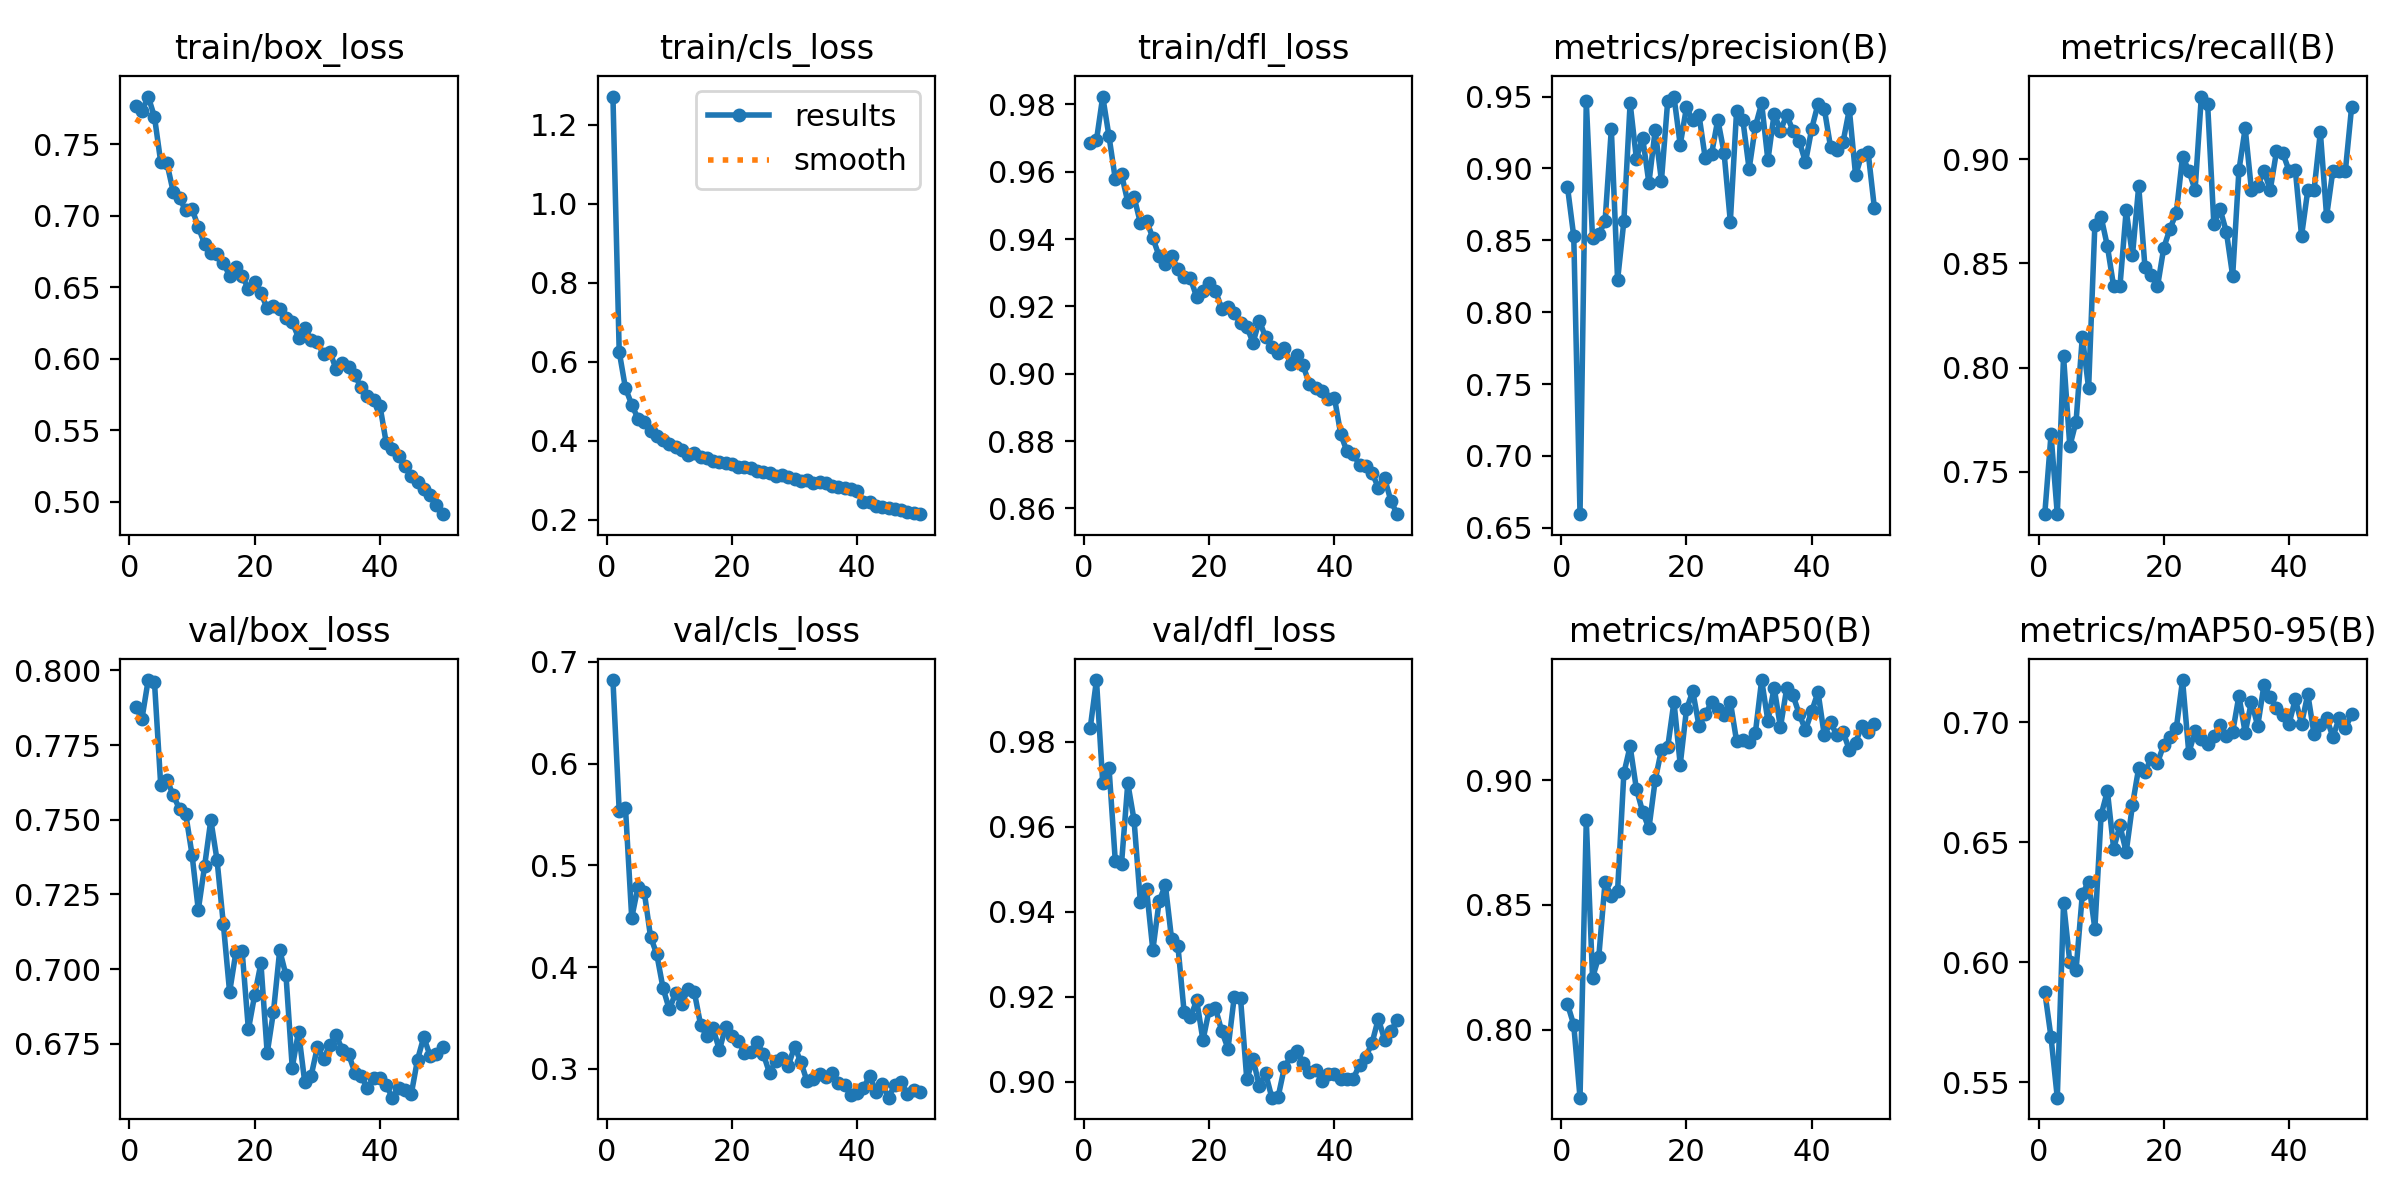
\includegraphics[width=0.55\textwidth]{data/training_results.png}
    \caption{Trainingsergebnisse des YOLOv5-Modells.}
    \label{fig:training}
\end{figure}

Zu erkennen ist, dass sowohl die Trainings- als auch Validierungsverluste (box\_loss, cls\_loss, dfl\_loss) im Verlauf kontinuierlich abnehmen, was auf ein stabiles und erfolgreiches Training hindeutet. Besonders der Klassifikationsverlust (cls\_loss) zeigt eine schnelle Konvergenz in den ersten zehn Epochen. Die Präzision und der Recall pendeln sich im oberen Bereich ein – teils mit leichten Schwankungen, die jedoch durch das kleine Modell und die geringe Batch-Größe erklärbar sind.\singlespacing

Besonders relevant ist der mean Average Precision (mAP) – ein Maß für die Genauigkeit bei verschiedenen IoU-Schwellenwerten. Der Wert mAP@0.5 steigt im Verlauf des Trainings auf über 0,9, während mAP@0.5:0.95 einen stabilen Endwert um 0,70 erreicht. Dies spricht für eine hohe Detektionsqualität, auch bei komplexeren Szenarien.
\paragraph{Konfidenz und Modellanwendung}
Die Ausgabe eines YOLO-Modells enthält neben den erkannten Objektpositionen auch sogenannte Konfidenzwerte, also Wahrscheinlichkeiten, mit denen das Modell ein Objekt als erkannt einstuft. In unserem Projekt wurde ein Konfidenzschwellenwert definiert, um falsch-positive Erkennungen zu reduzieren. Nur Detektionen mit einer Konfidenz über diesem Schwellenwert wurden weiterverarbeitet.\singlespacing

Das trainierte YOLOv5-Modell im .pt-Format wurde zur Performanzoptimierung in das NCNN-Format konvertiert. NCNN ist ein hochoptimiertes Inferenz-Framework speziell für mobile und eingebettete Systeme. Dadurch konnte das Modell auf dem Raspberry Pi 4 mit hoher Effizienz ausgeführt werden. Die Anwendung läuft in einem Skript, das serienweise acht Bilder aufnimmt und analysiert – was nahezu Echtzeitverarbeitung ermöglicht.

\paragraph{Einfluss der Trainingsdaten und Verbesserungsmöglichkeiten}
Die Qualität und Diversität der Trainingsdaten hat direkten Einfluss auf die Erkennungsleistung. In unserem Fall war der Datensatz breit gefächert, jedoch auf Kennzeichen fokussiert. Mögliche Optimierungen für die Zukunft wären:

\begin{itemize}
    \item Erweiterung des Datensatzes um reale eigene Aufnahmen
    \item Feinjustierung der Augmentierungstechniken
    \item Transfer Learning mit größeren Basismodellen
    \item Active Learning durch gezieltes Nachtraining mit fehlerhaften Beispielen
  \end{itemize}

  Dadurch könnte die Robustheit des Modells gezielt für Spezialfälle wie Nachtaufnahmen, verschmutzte Kennzeichen oder ungewöhnliche Kamerawinkel verbessert werden.


\subsubsection{Image Preprocessing}

Die Bildvorverarbeitung dient der Verbesserung der visuellen Eigenschaften der Bildausschnitte, in denen die Nummernschilder enthalten sind. Ziel ist es, die Zeichenstrukturen klar hervorzuheben, Bildrauschen zu minimieren und die Voraussetzungen für eine spätere Weiterverarbeitung, beispielsweise durch Texterkennung, zu schaffen.\singlespacing

Der erste Schritt der Pipeline besteht in der Umwandlung des Originalbildes in ein Graustufenbild. Dieses wird anschließend um den Faktor 3 vergrößert, um relevante Details, insbesondere feine Strukturen von Zeichen, deutlicher hervorzuheben. Im Anschluss erfolgt eine Glättung mittels eines Gaußschen Weichzeichners mit einer Kernelgröße von 3$\times$3, um Bildrauschen zu unterdrücken.

Darauf folgt ein binäres Thresholding mit inversierter Darstellung (\texttt{cv2.THRESH\_BINARY\_INV}). Durch diese Umkehrung erscheinen potenzielle Zeichenbereiche weiß auf schwarzem Hintergrund, was die spätere Konturerkennung erleichtert.\singlespacing

Um benachbarte Strukturen zu verbinden und kleinere Lücken in Zeichenformen zu schließen, wird im nächsten Schritt eine morphologische Dilation durchgeführt. Hierbei wird ein rechteckiges Strukturierungselement der Größe 3$\times$3 verwendet.\singlespacing

Die vorbereiteten Bilder werden im Anschluss zur Konturerkennung verwendet, wobei die Konturen in der Regel einzelnen Zeichen oder Zeichenkomponenten entsprechen. In späteren Verarbeitungsschritten können diese Bereiche gezielt extrahiert und analysiert werden.\singlespacing

Durch diese Kette an Vorverarbeitungsschritten wird sichergestellt, dass relevante Bildinformationen betont und störende Einflüsse reduziert werden, um die Qualität der anschließenden Bildanalyse zu maximieren.


\subsubsection{Optical Character Recognition}

Nach Abschluss der Bildvorverarbeitung, bei der die Kennzeichenbilder in eine geeignete Form gebracht wurden, erfolgt die Erkennung der enthaltenen alphanumerischen Zeichen mittels Optical Character Recognition (OCR). Zu Beginn des Projekts wurden dazu verschiedene OCR-Engines untersucht, darunter auch EasyOCR. Diese Deep-Learning-basierte Bibliothek liefert in vielen Anwendungsfällen gute Ergebnisse, zeigte jedoch im praktischen Einsatz auf ressourcenschwacher Hardware wie dem Raspberry Pi 4 deutliche Einschränkungen. Der hohe Speicherbedarf und die langen Inferenzzeiten verhinderten eine Echtzeitverarbeitung.\singlespacing

Im Vergleich dazu bot Tesseract eine deutlich geringere Systemlast bei gleichzeitig stabiler Erkennungsleistung. Besonders in unserem Anwendungsfall – kontrastreiche, segmentierte Kennzeichenbilder – erwies sich Tesseract als ausreichend genau. Durch gezielte Konfigurationsmöglichkeiten, wie die Beschränkung auf bestimmte Zeichensätze und Layout-Modi, ließ sich die Leistung zusätzlich optimieren. Aus diesen Gründen fiel die Entscheidung auf die Kombination aus Tesseract und der Python-Bibliothek \texttt{pytesseract}.\singlespacing

Im nächsten Schritt der Pipeline erfolgt eine Konturanalyse auf dem vorbereiteten binären Bild. Die erkannten Konturen werden nach verschiedenen geometrischen Kriterien gefiltert, um nur relevante Regionen weiterzuverarbeiten – etwa anhand von Größe, Seitenverhältnis und Position. Für jede verbleibende Kontur wird ein leicht vergrößerter Bildausschnitt (Region of Interest) definiert. Dieser wird an die OCR-Engine übergeben.\singlespacing

Die Texterkennung wird über die Funktion \texttt{image\_to\_data} durchgeführt. Dabei wird der zu analysierende Zeichensatz auf Großbuchstaben und Ziffern eingeschränkt (\texttt{tessedit\_char\_whitelist}) und mit dem Seitenlayout-Modus \texttt{--psm 8} gearbeitet, der für einzelne Zeichen geeignet ist. Das Ergebnis umfasst neben dem erkannten Text auch Positionsdaten und Konfidenzwerte.

Abschließend werden die erkannten Zeichenbereiche im Graustufenbild visuell hervorgehoben und als Bilddateien gespeichert, um die Ergebnisse nachvollziehbar und prüfbar zu machen.

\subsubsection{Herausforderungen bei realen Bedingungen}
Im Rahmen der Entwicklung unseres Kennzeichenerkennungssystems, das auf eine Mautstationssituation ausgelegt ist, traten verschiedene Herausforderungen auf, die unter realen Bedingungen von besonderer Bedeutung sind. \singlespacing

Eine der ersten Schwierigkeiten bestand in der Vielfalt von Kfz-Kennzeichen weltweit. 
Während die Objekterkennung des Kennzeichens selbst (die Lokalisierung auf dem Bild) zuverlässig funktionierte, erwies sich das anschließende Auslesen der Schriftzeichen als problematisch. 
 Dies lag an den unterschiedlichen Formaten, Schriftarten und Normen, die international variieren. 
 Nach eingehender Analyse kamen wir zu dem Entschluss, dass die Entwicklung eines universellen Kennzeichenerkenners, der alle internationalen Standards abdeckt, den Rahmen unseres Projektes deutlich überschreiten würde. 
 Stattdessen entschieden wir uns, eine optimierte Lösung speziell für deutsche Kfz-Kennzeichen zu entwickeln, um innerhalb der gegebenen Projektgrenzen eine funktional stabile Erkennung zu gewährleisten.\singlespacing
 Eine weitere Herausforderung stellte die Anpassung des Systems an verschiedene Licht- und Schattenbedingungen dar. 
 Schon bei kleinen aber vor allem bei stark wechselnden Beleuchtungsverhältnissen war die Festlegung geeigneter Thresholds bei der Bildverarbeitung für eine universale Lösung herausfordernd. 
 Auch hier zeigte sich, dass eine umfassende allgemeine Lösung, die alle möglichen Umgebungsbedingungen robust abdeckt, einen erheblichen zusätzlichen Entwicklungsaufwand erfordern würde. \singlespacing
 Zudem stießen wir auf technische Grenzen hinsichtlich der Leistungsfähigkeit des eingesetzten Raspberry Pi.
Insbesondere die Schriftzeichenerkennung stellte hohe Anforderungen an die Prozessorleistung, was die Echtzeitfähigkeit des Systems deutlich beeinträchtigte.
Es wurde schnell klar, dass der Raspberry Pi vor allem für den Einsatz unter kontrollierten Laborbedingungen geeignet ist, während für Anwendungen unter realen Bedingungen leistungsstärkere Hardware empfohlen wird.
Die Herausforderung lag hier insbesondere darin, eine akzeptable Balance zwischen Hardwareanforderungen und Systemleistung herzustellen.\singlespacing

Vor diesem Hintergrund entschieden wir uns bewusst für die Verwendung der YOLOv5-Architektur, da diese im Vergleich zu neueren Modellen wie YOLOv8 eine deutlich geringere Rechenlast aufweist und damit besser auf ressourcenbeschränkter Hardware wie dem Raspberry Pi lauffähig ist.
Die Wahl eines leichteren Modells ermöglichte es, die grundlegenden Funktionen der Gesichts- und Schrifterkennung trotz der beschränkten Systemressourcen zuverlässig zu demonstrieren. 
\subsubsection{Optimierung für wechselnde Lichtverhältnisse und Kameraperspektiven}
\subsubsection{Evaluation und Genauigkeitsanalyse}

\subsection{Gesichtserkennung}
\subsubsection{Testaufbau}
Das implementierte System realisiert eine Echtzeit-Gesichtserkennung mittels einer handelsüblichen Webcam (640$\times$480 Pixel) und verwendet das Modell \texttt{YOLOv8n-face} zur Detektion von Gesichtern. Die Identifikation erfolgt durch Kombination der YOLO-basierten Gesichtserkennung mit dem \texttt{face\_recognition}-Framework, das HOG-basierte Merkmalsextraktion nutzt. Bekannte Gesichter werden im lokalen Verzeichnis gespeichert und können über eine grafische Benutzeroberfläche dynamisch erweitert werden. Das System ist für Zutrittskontrollszenarien konzipiert und erlaubt das Anlernen neuer Gesichter im laufenden Betrieb.

\subsubsection{YOLO}
\paragraph{Vergleich der YOLO-Modelle}
\begin{table}[h]
    \centering
    \begin{tabular}{|l|c|c|c|c|l|}
    \hline
    \textbf{Modell} & \textbf{mAP (face)} & \textbf{Inferenzzeit (ms)} & \textbf{Parameter} & \textbf{FLOPs} & \textbf{Besonderheiten} \\
    \hline
    YOLOv8n-face   & 39{,}2\%   & 80{,}4   & 3{,}2 Mio. & 8{,}7 Mrd. & Auf Gesichtserkennung spezialisiert \\
    YOLOv8n        & 37{,}3\%   & 80{,}4   & 3{,}2 Mio. & 8{,}7 Mrd. & Generelles Objekterkennungsmodell   \\
    YOLOv11n-face* & 41{,}5\%*  & 56{,}1   & 2{,}6 Mio. & 6{,}5 Mrd. & Verbesserte Architektur, schneller  \\
    \hline
    \end{tabular}
    \caption{Vergleich der wichtigsten YOLO-Modelle für die Gesichtserkennung. *Werte für YOLOv11n-face sind geschätzt, basierend auf aktuellen Trends in der YOLO-Architektur.}
    \end{table}
    
    Das auf Gesichter spezialisierte Modell YOLOv8n-face erzielt eine höhere Genauigkeit als das generische YOLOv8n. Das neuere YOLOv11n-face bietet voraussichtlich noch bessere Erkennungsraten und eine deutlich schnellere Inferenz, erfordert jedoch ggf. Anpassungen und erneutes Training für die Kompatibilität mit dem aktuellen Code. Generische Modelle wie YOLOv8n erkennen mehr Objekttypen, sind aber für die reine Gesichtserkennung weniger effizient.

\paragraph{Metriken}
Für die Bewertung der Gesichtserkennung sind folgende Metriken relevant:
\begin{itemize}
    \item \textbf{Precision (Genauigkeit):} Anteil der korrekt erkannten Gesichter an allen als erkannt gemeldeten Gesichtern.
    \item \textbf{Recall (Sensitivität):} Anteil der korrekt erkannten Gesichter an allen tatsächlich vorhandenen Gesichtern.
    \item \textbf{F1-Score:} Harmonisches Mittel aus Precision und Recall.
    \item \textbf{Inferenzgeschwindigkeit:} Anzahl der Bilder pro Sekunde (FPS) bzw. durchschnittliche Latenz pro Bild.
\end{itemize}

\paragraph{Python-Code zur Visualisierung}
%Python Diagramm

Zur Auswertung können folgende Attribute der \texttt{ultralytics}-Bibliothek genutzt werden:
\begin{itemize}
    \item \texttt{results.box.map50} für mAP@0.5 (mean Average Precision)
    \item \texttt{results.speed} für Inferenzzeit (ms pro Bild)
\end{itemize}

\paragraph{Anwendungsbeispiel: Zutrittskontrollen}
Das System ermöglicht eine zuverlässige Gesichtserkennung für Zutrittskontrollsysteme mit folgenden Eigenschaften:
\begin{itemize}
    \item Echtzeit-Erkennung mit einer Latenz von unter 250\,ms pro Bild.
    \item Visuelles Feedback durch Markierung und Beschriftung erkannter Gesichter im Videostream.
    \item Dynamisches Anlernen neuer Nutzer durch interaktive Eingabe.
    \item Speicherung der Gesichtsdaten in einem lokalen Verzeichnis; Erweiterung durch SQLite möglich.
    \item Erweiterbar für Multi-Faktor-Authentifizierung (z.\,B. RFID + Gesicht).
\end{itemize}

\textbf{Ergebnisse:} In kontrollierter Umgebung erreicht das System eine Erkennungsrate von ca.~93\,\%. Bei schwierigen Lichtverhältnissen sinkt die Rate auf etwa 78\,\%. Für produktive Anwendungen empfiehlt sich die Ergänzung durch IR-Kameras und Liveness Detection.

\begin{quote}
Das vorgestellte System kombiniert die Geschwindigkeit und Präzision moderner YOLO-Modelle mit der Flexibilität des Face-Recognition-Frameworks und ist damit für den Einsatz in sicherheitskritischen Zutrittskontrollen geeignet.
\end{quote}

\subsubsection{MediaPipe}
\paragraph{Gesichtspunkterkennung}


\paragraph{Gesichtswiedererkennung mit Gesichtspunkten}

\paragraph{Metriken}
Für die Bewertung der Gesichtspunkterkennung mit MediaPipe sind folgende Metriken relevant:
\begin{itemize}
    \item \textbf{Failure Rate:} Anteil der Bilder, bei denen kein Gesicht erkannt wurde.
    \item \textbf{Landmark Error:} Durchschnittlicher Fehler bei der Lokalisierung der Gesichtspunkte.
    \item \textbf{Confidence Score:} Wahrscheinlichkeit, dass ein Gesicht erkannt wurde.
    \item \textbf{Inferenzgeschwindigkeit:} Anzahl der Bilder pro Sekunde (FPS) bzw. durchschnittliche Latenz pro Bild.
\end{itemize}


\textbf{Failure Rate} \\


\textbf{Confidence Score} \\


\textbf{Inferenzgeschwindigkeit} \\

Die Augfabenstellung umfasste die Analyse und Bewertung die Performance der MediaPipe Gesichtserkennung und Gesichtswiedererkennung hinsichtlich ihrer Inferenzgeschwindigkeit und Stabilität.

Für die Gesichtserkennung wurden für verschiedene Confidence-Werte (50\% und 80\%) die FPS (Frames per second), Verarbeitungszeit und die Stabilität berechnet und verglichen.

Die Gesichtswiedererkennung wurde mit dem MediaPipe FaceMesh auf einer einheitlichen Webcam-Auflösung (640 auf 480) durchgeführt. Über einen Zeitraum von 60 Sekunden wurden in 5-Sekunden-Intervallen FPS, durschnittliche Verabeitungszeit pro Frame, erkannte Gesichter sowie ein Stabilitätswert berechnet und dokumentiert.
Für die Confidence-Werte von 50\% und 80\% wurde jeweils ein separater Test durchgeführt.

Die Ergebnisse zeigen deutlich, dass eine Erhöhung des Confidence-Schwellenwerts von 50\% auf 80\% einen signifikanten Einfluss auf die Inferenzgeschwindigkeit hat. Bei einem Confidence-Wert von 50\% wurde eine durchschnittliche Framerate von 27.16 FPS mit einer mittleren Verarbeitungszeit von 8.81 ms pro Frame erreicht. Im Gegensatz dazu sank die durchschnittliche FPS bei einem Confidence-Wert von 80\% auf 20.6, während die mittlere Verarbeitungszeit auf 12.68 ms anstieg. Dies deutet darauf hin, dass ein höherer Confidence-Wert zu einer genaueren, aber auch langsameren Verarbeitung führt, da das Modell länger nach sichereren Erkennungen sucht.

Die Stabilität der Gesichtserkennung blieb in beiden Tests mit durchschnittlich 97.73\% (bei 50\% Confidence) und 99\% (bei 80\% Confidence) relativ hoch. Dies deutet darauf hin, dass die Erkennung über die Zeit hinweg zuverlässig Gesichter identifizieren konnte, wobei der höhere Confidence-Wert tendenziell zu einer noch stabileren Erkennung führte.

Die Beobachtungen während der Tests bestätigen, dass die Leistung der MediaPipe Gesichtserkennung von verschiedenen Faktoren beeinflusst wird. Eine höhere Anzahl von Gesichtern, eine bessere Auflösung des Eingabebildes und ein höherer Confidence-Wert scheinen die Verarbeitungszeit zu erhöhen und die FPS zu reduzieren. Zudem ist die Leistung erwartungsgemäß von der Hardware des verwendeten Geräts abhängig. Trotz dieser Schwankungen zeigte sich die Erkennung als recht stabil, ohne signifikante Ausreißer in den Leistungswerten über die Zeit, was auch in Abbildung \ref{fig:fps_ueber_zeit} visualisiert wird. Es ist jedoch anzumerken, dass die Stabilität auch von der Bewegung der erfassten Person abhängen kann, was in den vorliegenden Tests nicht explizit variiert wurde.

Die Gegenüberstellung der Leistung bei unterschiedlichen Confidence-Werten in Abbildung \ref{fig:vergleich_confidence} verdeutlicht den Trade-off zwischen Geschwindigkeit und Konfidenz. Die Wahl des optimalen Confidence-Werts hängt somit stark von der jeweiligen Anwendung ab, bei der entweder eine hohe Geschwindigkeit oder eine hohe Sicherheit der Erkennung priorisiert wird.

\begin{figure}[ht]
    \centering
    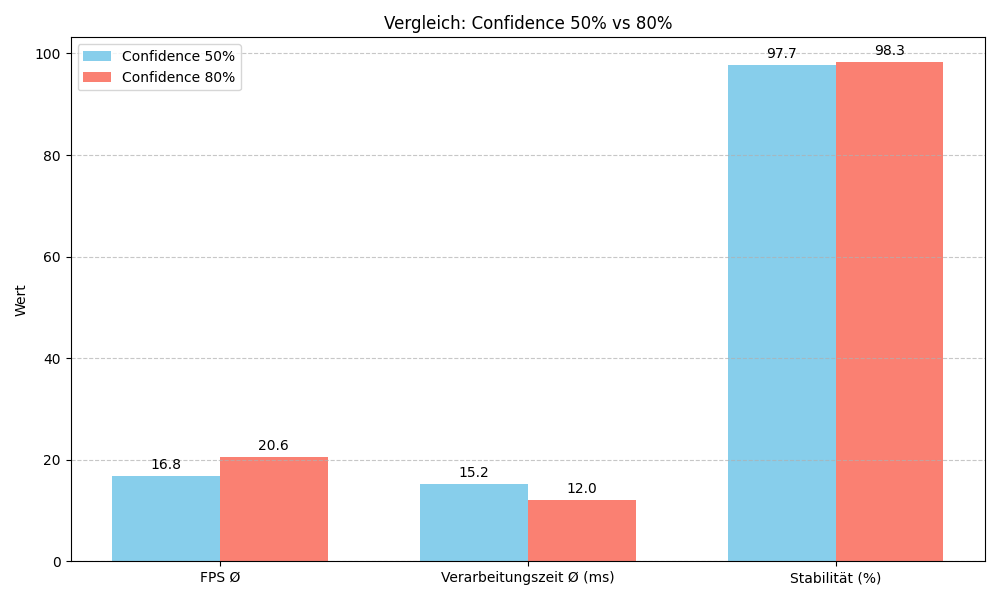
\includegraphics[width=0.55\textwidth]{data/Vergleich_Confidence_50_vs_80.png}
    \caption{Vergleich der Confidence-Scores.}
    \label{fig:vergleich_confidence}
\end{figure}


\begin{figure}[ht]
    \centering
    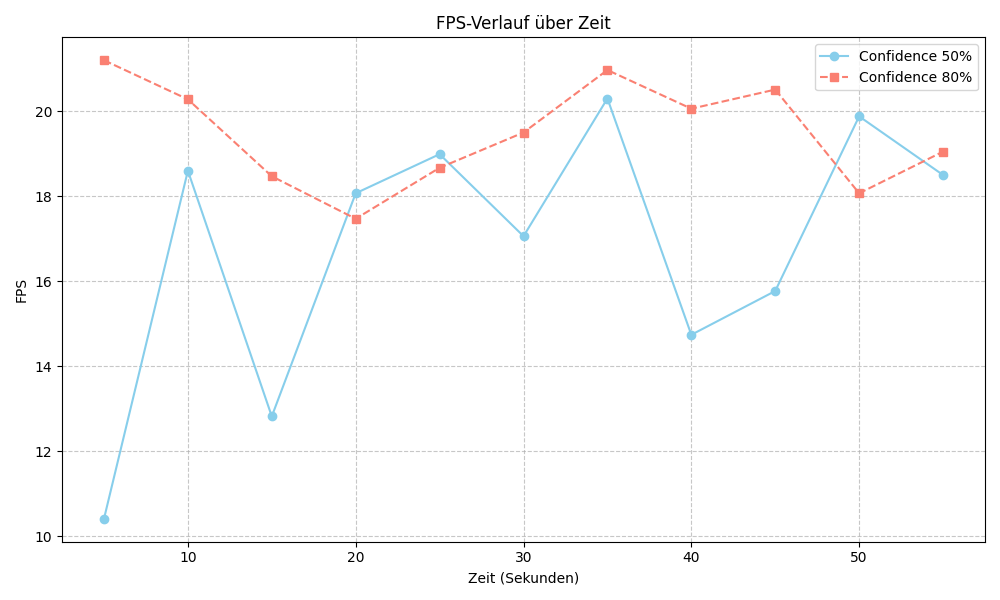
\includegraphics[width=0.55\textwidth]{data/FPS_ueber_Zeit.png}
    \caption{FPS-Werte über Zeitspanne von 60 Sekunden.}
    \label{fig:fps_ueber_zeit}
\end{figure}


\paragraph{Metriken}
\paragraph{Anwendungsbeispiel: Zutrittskontrollen}

\subsubsection{Vergleich}
\paragraph{Confidence Score}
\paragraph{FPS / Inference Time}

\subsubsection{Manipulierte Gesichtserkennung}
\paragraph{Angriffsmethoden auf Gesichtserkennungssysteme}
\paragraph{Testen der Robustheit gegen Manipulationen}
\paragraph{Möglichkeiten zur Absicherung}

\subsubsection{Projektdokumentation}
\paragraph{Vorgehensmodell und Teamorganisation}
\paragraph{Dokumentation des Projektmanagements}